\documentclass[english, a4paper, 12pt, twoside]{book}

% -------------- Setup, do not change these ---------------
\usepackage{textcomp}
\usepackage[T1]{fontenc, url}
\usepackage[utf8]{inputenc}
\usepackage{titlesec}
\setcounter{secnumdepth}{4}
\usepackage{multirow}
\usepackage{braket}


\usepackage{adjustbox}
\usepackage{graphicx}
\usepackage{amsmath, amssymb, amsthm} % Mathematical packages
\usepackage{parskip} % Removing indenting in new paragraphs
\urlstyle{sf}
\usepackage{color}
\usepackage{subcaption}
\usepackage{appendix}
\usepackage{chngcntr} % needed for correct table numbering
\counterwithin{table}{section} % numbering of tables
\counterwithin{figure}{section} % numbering of figures
\numberwithin{equation}{section} % numbering of equations
\hyphenpenalty=100000 % preventing splitting of words
\sloppy
\raggedbottom
\usepackage{xparse,nameref}
\usepackage[bottom]{footmisc} % Fotnotes are fixed to bottom of page


% --------- You can edit from this point on --------


% ----- Appearance and language -----
\usepackage[english]{babel} % document language
\graphicspath{{./img/}} % path to images
\usepackage[margin=2.54cm]{geometry} % sets margins for the document
\usepackage{setspace}
\linespread{1} % line spread for the document
\usepackage{microtype}


% ----- Sections -----
\titleformat*{\section}{\LARGE\bfseries} % \section heading
\titleformat*{\subsection}{\Large\bfseries} % \subsection heading
\titleformat*{\subsubsection}{\large\bfseries} % \subsubsection heading
% next three lines creates the \paragraph command with correct heading
\titleformat{\paragraph}
{\normalfont\normalsize\bfseries}{\theparagraph}{1em}{}
\titlespacing*{\paragraph}
{0pt}{3.25ex plus 1ex minus .2ex}{1.5ex plus .2ex}


% ----- Figures and tables -----
\usepackage{fancyhdr}
\usepackage{subfiles}
\usepackage{array}
\usepackage[rightcaption]{sidecap}
\usepackage{wrapfig}
\usepackage{float}
\usepackage[labelfont=bf]{caption} % bold text for captions
\usepackage[para]{threeparttable} % fancy tables, check these before you use them
\usepackage{url}
\usepackage[table,xcdraw]{xcolor}
\usepackage{makecell}
\usepackage{hhline}
\usepackage{booktabs}

\usepackage[breaklinks=true,colorlinks=true,linkcolor=black,urlcolor=blue,citecolor=blue]{hyperref}
% ----- Sources -----

%\bibliographystyle{apa} % citation and reference list style
%\def\biblio{\clearpage\bibliographystyle{apa}\bibliography{References.bib}} % defines the \biblio command used for referencing in subfiles - DO NOT CHANGE


% ----- Header and footer -----
\pagestyle{fancy}
\fancyhead[RO,LE]{\thepage} % page number on right for odd pages and left for even pages in the header
\fancyhead[RE,LO]{\nouppercase{\rightmark}} % chapter name and number on the right for even pages and left for odd pages in the header
%\renewcommand{\headrulewidth}{0pt} % sets thickness of header line
\fancyfoot{} % removes page number on bottom of page


% ----- Header of the frontpage -----
\fancypagestyle{frontpage}{
	\fancyhf{}
	\renewcommand{\headrulewidth}{0pt}
	\renewcommand{\footrulewidth}{0pt}
	\vspace*{1\baselineskip}

	%\fancyhead[R]{Norwegian School of Economics
	%\linebreak       Bergen, Fall 2018\vspace*{5\baselineskip}}
	\fancyhead[C]{ \includegraphics[width=3.5in]{img/logo}}
}


% ----- Document starts here -----
\begin{document}

%\def\biblio{} % resets the biblio command, if not here a new reference list will be produced after every chapter
{\setstretch{1.5}

\begin{titlepage}

 \newgeometry{top=1 in, bottom=1 in, left=1 in, right= 1 in}

 \thispagestyle{frontpage}

 \begin{center}

   \vspace*{6\baselineskip}


   {\Huge \textbf{A single-ion-focused 393$\,$nm laser for photon generation and qubit control\\}}



       \vspace*{1,5\baselineskip}


   \vspace{1,5\baselineskip}

   \large{A master’s thesis submitted to the faculty of mathematics, computer science and physics, of the University of Innsbruck\\ in partial fulfillment of the requirements for the degree of\\\vspace{1,2\baselineskip}\textbf{Master of Science (MSc)} \\\vspace{1,2\baselineskip}carried out at the Institute of Experimental Physics under the supervision of}\\
   \large{o.Univ.-Prof.  Dr.  Rainer Blatt,}\\
   \large{Dr. Ben Lanyon}\\
    \vspace{1,2\baselineskip}
   \large{Presented by\\}
   \huge{\textbf{Marco Canteri}}\\
   \vfill
   \large{ }

 \end{center}

\end{titlepage}

}
\restoregeometry % restores the margins after frontpage
%\nocite{*} % uncomment if you want all sources to be printed in the reference list, including the ones which are not cited in the text

\pagenumbering{gobble} % suppress page numbering
\thispagestyle{plain} % suppress header
\clearpage\mbox{}\clearpage % add blank page

\pagenumbering{roman} % starting roman page numbering
\newpage

\section*{Abstract}
I swear I did something

\newpage


\newpage
\tableofcontents


\newpage
\addtocontents{toc}{\protect\setcounter{tocdepth}{4}} % sets depth of toc to 4, 1.1.1.1
\pagenumbering{arabic} % Starting arabic page numbering
\setcounter{page}{1} % sets pagecounter to 1

\chapter{Introduction} % section/chapter name

Quantum computing has been a rapidly increasing field of interest, which is probably due to the fact that it represents the
next step in technology advancement. Classical computers are limited in solving some particular problems that scale exponentially, and therefore a new approach is needed. Quantum computing can exploit particular features of quantum mechanics that have no classical counterparts, this allows for a speed up for a certain class of problems such as factorizing numbers \cite{shor}, or searching in a database \cite{grover}. Moreover, simulating nature at its quantum level is a hard task for classical computer, while quantum computers are naturally prone to simulate quantum dynamics.\\
A set of criteria exists to assess the viability of a realistic implementation of a quantum computer \cite{divincenzo}, several platforms have been proposed and implemented trying to satisfy these criteria. Ion trapping has already fulfilled all criteria experimentally and it shows great potential for a possible large scale quantum computer. The idea is simple, qubits are encoded in the electronic state of single trapped ions in a Paul trap. Manipulation can be done easily with laser pulses and by placing a cavity, an ion trap gains network abilities.\\
However, still a lot of challenges needs to be addressed for a quantum computer to outperform a classical one. Due to the incredible delicate nature of qubits, they are subject to decoherence which harms the successfulness and computational power of quantum computers. Therefore, scaling the number of qubit has been proven to be a difficult engineeristic challenge. Several solutions are possible: the number of qubits can scale; the dimension of qubits can decrease; or qubits can be linked together. The last solution is the approach at the base of quantum networks. The idea is to connected several quantum computers to create a cluster of nodes that can work jointly. The task of building a quantum network is not trivial, there are fundamental difference with a classical link. Although the mean can be the same, such as optical fiber, a quantum network must have additional abilities, such as distributing entanglement, or transmitting quantum states. In addition to scaling quantum computers, quantum networks allow for more secure transmission of information \cite{qkd}, and improve some measurements \cite{quantumclocks}.\\
It is in this context that this thesis arises. Currently there is an ongoing project of building a three node quantum network between two buildings on the campus of the University of Innsbruck. The third node is located in IQOQI, where the thesis took place. Here an ion trap is used as node of the network and it is connected with a 400m fiber link. The 393nm lasers is responsible for the generation of the transmitted photons via a cavity enhanced Raman process. At the time of this thesis' start, the 393nm laser was shining in the whole trap. In this case, if an ion string were to be loaded, the light would hit all the ions equally and there would be no control over the single ion-photon pair. This limits the experiments and the production of photons to one single ion.\\
To overcome this limitation, an optical setup for the 393nm laser had to be built with the purpose of focusing the light to a single ion in a string. Moreover the setup should have the ability to steer the beam and focus it on a different ion. The goal of this thesis was indeed to design and build such a system. The setup is per se not complex, but the design is critical, ions separation is typical in the order of $\mu$m, which means the light should be focused down to $1-2\,\mu$m, at the limits of the optical elements involved. The steering part is achieved with an acousto-optical deflector (AOD), such device deflects the laser light proportionally to the applied input frequency allowing to control remotely the beam ponting of the system.\\
 Once completed, the system will allow to manipulate single ions in a string. The same laser can manipulate ions in two different ways: we already mentioned the most important: the triggering of the photon's generation; but, by driving in the laser in a different regime, it is also possible to implement a single qubit gate. This is used to implement quantum operations that are the base for some experiments. For instance, the characterization and beam shape probing experiment performed in this thesis is built on top of such quantum operation.\\
 \newline
 This work is presented in the following way: Chapter 2 is devoted to the theoretical background necessary to understand the rest of the work. Here the foundations of quantum computing and networking are laid down, along with the basic concepts of ion trapping; Chapter 3 presents the existing experimental setup, i.e. the already built and working blocks of the experiment where the setup designed in this thesis has been added; Chapter 4 is the core of the thesis, here the final design made with the software Zemax and simulations of different aspects of the project are introduced and presented;
Chapter 5 contains all the experimental results obtained. It is divided in two parts: First, the setup was built on a spare optical table, here we had the freedom to test the performance of the system under different aspects and decide whether or not it was satisfactory. After having the certainty that the system will work, the setup was transferred and aligned on the real experiment where limited access did not consent for easy performance testing. Here, different and more complicated experimental methods had to be used to check if the system was working properly. The description and discussion of these results are in the second part of chapter 5.


% Theory chapter
\chapter{Theoretical framework}
Quantum computing is based on a general framework that does not depend on the physical platform. Here, important concept such as qubit, and quantum operations are described before showing how we can realize them, from a theoretical point of view, with trapped ions. The same goes with quantum networking, the concept and the realization can be treated separately and they will be described in this chapter. Furthermore, in this chapter we will take a look into Gaussian beams and their properties. Since that is the shape emitted by laser, it is important to understand their characteristic and how to manipulate them. Lastly Acousto-optical interactions are introduced and studied to give an idea of how AODs work and how they can be used to steer a laser beam.
\section{Quantum logic with trapped ions}
\subsection{Quantum computer and quantum gates}
The concepts of quantum computing are borrowed and extended from classical computational theory. In the classical case, information is represented in terms of binary digits, the so called bit, essentially mapping information to a base-2 number. Information processing is done with gates acting of those numbers. The idea of quantum computer is still to encode information in a binary form, but due to the nature of quantum mechanics, a quantum bit (in short qubit) gains new features that can be exploited to perform different kind of operations that in some cases are a speed up compared to the classical case.\\
A qubit is formally a normalized wave function that can be written as superposition of two orthogonal states indicated usually with $\ket{0}$ and $\ket{1}$:
\begin{equation}
\label{qubit}
\ket{\psi} = \alpha \ket{0} + \beta\ket{1},
\end{equation}
where $\alpha,\beta$ are probability amplitudes, two complex numbers that satisfy the relationship $|\alpha|^2+|\beta|^2 = 1$.
At first glance, the advantage of qubits seems obvious, while one classical bit can store only one bit of information, a qubit can be in any linear combination, i.e. $\alpha$ and $\beta$ can be chosen freely and any information can be represented. Although, the reality is different, due to rules of quantum mechanics, $\alpha$ and $\beta$ cannot be directly accessed, which means that we can get only a limited amount of information out of a qubit. The outcome of measuring a qubit will give the value 0 with a probability of $|\alpha|^2$ and 1 with a probability of $|\beta^2|$.  [..]

Qubits also have a geometrical representation that can be useful, equation \eqref{qubit} depends on 4 real numbers, however since $\psi$ is normalized, we can rewrite the expression as
\begin{equation}
\ket{\psi} = e^{i\gamma}\left(\cos\frac{\theta}{2}\ket{0} + e^{i\varphi}\sin\frac{\theta}{2}\ket{1}\right).
\end{equation}
the global phase factor $e^{i\gamma}$ can be left out, as it does not influence the measurement outcome. This leaves us with only two real number: $\theta$ and $\varphi$. A qubit is therefore representable with only these two numbers that we can chose to represent geometrically with normalized spherical coordinates. The so called Bloch sphere is depicted in figure \ref{blochsphere}, every point on its surface represents a different state of the qubit. Here qubit manipulation can be visualized as trajectories on the surface, which in some cases is very useful. The drawback of this representation is that it is limited to only one qubit, so it loses usefulness when dealing with multiple qubits.
\begin{figure}[H]
\centering
\includegraphics[width = .4\textwidth]{bloch_sphere}
\caption{The Bloch sphere. The states $\ket{0}$ and $\ket{1}$ are at the poles of the sphere, every other point of the surface represents a superpositions of these states. A quantum gate can be seen as trajectory on the surface mapping one state to another.}
\label{blochsphere}
\end{figure}

A more practical way of dealing with qubits is via matrices. We can assign to the states $\ket{0}$ and $\ket{1}$ the following:
\begin{equation}
\ket{0} = \begin{pmatrix}
 1 \\
 0
\end{pmatrix} \quad
\ket{1} = \begin{pmatrix}
 0 \\
 1
\end{pmatrix} \implies \ket{\psi} = \begin{pmatrix}
 \alpha \\
 \beta
\end{pmatrix}.
\end{equation}
In this representation, manipulations of qubits are easily calculated using $2\times2$ unitary matrices. These kind of operations are named \emph{quantum gates} and they are the building blocks of quantum computing. Every quantum algorithm can be written as a sequence of quantum gates and it is therefore important to understand them. For a single qubit any gate can be written as combination of two operations \cite{hempel}
\begin{equation}
U_z(\theta) =  \begin{pmatrix}
 e^{-i\frac{\theta}{2}} & 0 \\
 0 & e^{i\frac{\theta}{2}}
\end{pmatrix} \qquad U_\varphi(\theta) = \begin{pmatrix}
\cos\frac{\theta}{2} & -i e^{-i\varphi}\sin\frac{\theta}{2} \\
-ie^{i\theta}\sin\frac{\theta}{2} & \cos\frac{\theta}{2}
\end{pmatrix}.
\end{equation}
These two matrices can be seen as two different rotations in the Bloch sphere, $U_z$ is a rotation around the $z$ axis by the amount $\theta$, while $U_\varphi$ is a rotation on the $x-y$ plane around an axis tilted by $\varphi$. examples [H gate, phase gate]\\
\newline
As we have seen, a single qubit has already the advantage of superposition compared to classical case. When considering multiple qubits, we gain even more quantum mechanical features like entanglement. This phenomenon does not have a classical analogy and it is an extremely useful tools in quantum information.\\
In general a state with $N$ qubits is written as tensor product of the single qubit states $\psi_i$
\begin{equation}
\ket{\psi_N} = \ket{\psi_1}\otimes \ket{\psi_2}\otimes \cdots \ket{\psi_N} \equiv \ket{\psi_1\psi_2\dots \psi_N}.
\end{equation}
If we had to write out explicitly all the probability coefficients of $\psi_N$, we would need $2^N$ complex numbers. It is clear then why classical computer cannot keep up. $N$ bits can only give $N^2$ different combinations, while the Hilbert space of qubits is exponentially larger.\\
Now, let us consider only 2 qubits, a particular case would be
\begin{equation}
\ket{\psi} = \frac{1}{\sqrt{2}}\left(\ket{00} + \ket{11}\right).
\end{equation}
If a measurement is made on one of the two qubit and, for instance, the outcome is 0, the wave function collapses to the state $\ket{00}$, collapsing also the state of the other qubit, even if no operation has been directly performed on it. Next you measure the the second qubit and the outcome will be 0 with unitary probability. Viceversa, if the outcome if the first measurement was 1, the state collapses to $\ket{11}$ and the outcome of the second measurement is always 1. The two qubits are correlated, but this correlations is stronger than the classical one.\\
Gates that involve multiple qubits are written as $2^N\times 2^N$ unitary matrices, a famous example is the CNOT gate, [..]

It can be shown [] that the examples we saw here, H gate, phase gate, and CNOT gate form a universal set of quantum gates, i.e. a sequence of these gates approximate every other quantum gate.

\subsection{Ion qubits and laser-ion interactions}
Qubits can be encoded in any pair of orthogonal states. In the case of an ion it is possible to take two internal electronic states. The choices are multiple: an optical qubit is implemented in an optical transition, an hyperfine qubit is between two hyperfine states, and a Zeeman qubit can be realized with two magnetically separated levels. We will take the choice of an optical qubit, in this case lasers provide an easy way to manipulate the population of the two level and therefore to manipulate the state of the qubit, implementing quantum gates in an almost straightforward way. As long as the chosen levels are well separated, and the light is near resonant to the transition, it is possible to describe the system with the basic 2-level atom scheme interacting with classical light. \\
In this section, the theoretical model of a 2-level atom is presented together with a model of interactions between the laser and the ion. This represents a physical implementation of the concepts illustrated in the previous section.
\begin{figure}[H]
\centering
\includegraphics[width = .4\textwidth]{2levelatom}
\caption{2-level atom scheme, the ground and excited states are denoted as $\ket{g}$, and $\ket{e}$. $\omega_l$ is the laser frequency, which is detuned by $\Delta$ from the transition frequency $\omega_0$.}
\label{2levelatom}
\end{figure}

Consider the system in figure \ref{2levelatom}, the Hamiltonian of the atomic part can be written as:
\begin{equation}
H_a = \hbar\omega_0 \ket{e}\bra{e},
\end{equation}
where $\omega_0$ is the frequency difference between the ground and excited state, the energy of the ground state has also been set to 0. The Hamiltonian of the interaction between light and atom can be written as []
\begin{equation}
H_{int} = -d\cdot E
\end{equation}


- 2 level atom scheme\\
- Model of laser-ion interaction: rabi flops, AC stark shift
\section{Quantum networking with trapped ions}
\subsection{General introduction}
- Nodes, interface, link, protocols\\
- logic, memory, interface, Bell pairs, purification, multi-mode
- Distributed entanglement
\subsection{Cavity QED}
- Simple model atom in cavity: g,gamma, k
\section{Basics of ion trapping}
\subsection{Linear Paul trap}
- How a Paul trap works\\
- micromotion?
\subsection{Ion strings}
We have seen that the potential inside the trap can be described as an harmonic potential. It is then possible to calculate the ion separation between $N$ ion loaded in the trap. This will give us an idea of how narrowly the beam should be focused and will set an appropriate problem spatial scale.\\
We will consider only the $z$ direction where the ions are weakly confined and will form a string. The harmonic potential is then given by
\begin{equation}
V = \sum_{i=0}^N \frac{1}{2}M\omega^2z_i^2 + \sum_{i\neq j}^N\frac{Z^2e^2}{8\pi \epsilon_0}\frac{1}{|z_i-z_j|}
\end{equation}
The equilibrium position can be found at the minima of the potential, i.e. where the first derivative zeros
\begin{equation}
\frac{\partial V}{\partial z_i} = 0 \implies u_i - \sum_{j=1}^{i-1} \frac{1}{(u_i-u_j)^2} + \sum_{j= i+1}^{N} \frac{1}{(u_i-u_j)^2}= 0,
\end{equation}
where we defined the dimensionless quantity $u_i = z_i/l$ and $l^3 = \displaystyle\frac{Z^2 e^2 }{4\pi \epsilon_0 M\omega^2}$.
The last equations can be solved analytically only for 2 or 3 ions. In fact, for the case $N=2$ we simply get the system
\begin{equation}
\begin{cases}
  u_1 + \frac{1}{(u_1-u_2)^2} = 0\\
  u_2 - \frac{1}{(u_1-u_2)^2} = 0
  \end{cases} \quad \implies \quad u_1 = -u_2,\quad  u_1 = \left(\frac{1}{2}\right)^{2/3} \simeq 0.629
\end{equation}
For calcium-40 ions in a Paul trap with axial confinement of 1MHz, we have $l \simeq 4.45\times 10^{-6}\, \mu$m, which means that 2 ions are separated by $\simeq 5.6\, \mu$m. In the case of more ions the separation is lesser with the same confinement, but it is also possible to lower the axial frequency and increase the separation between the ions such that also in the case of several ions, the distance between them is still in the order of several $\mu$m. This size is accessible with current focusing optics and it is above the diffraction limit.\\
For more ions, a numerical approach has to be used, \cite{ion_spacing} reports values of $u_i$ up to $N=10$, and gives an empirical formula of the minimum separation
\begin{equation}
u_{min}(N) \simeq \frac{2.018}{N^{0.559}}
\end{equation}
\subsection{Doppler cooling and detection}
\section{Laser beam}
\subsection{Gaussian beams}
Lasers emit light in the shape of Gaussian beams, so it is import to understand what Gaussian beams are and their characteristics. In this chapter we will take a closer look into such beams and introduce important quantities to characterize a Gaussian beam. \\
From a theoretical point of view, Gaussiam beams are solution of the Helmholzt equation
\cite{saleh}
- Introduction to import quantities, like FWHM, focus, waist!
\subsection{Diffraction limit}
- To search whats limiting the diffraction, (lambda/2)
\subsection{Beam stearing via AOD's}
- How AODs work, simple Model\\
- Introduce diffraction efficiency, bandwidth


%Existing experimental setup chapter
% !TEX root = main.tex

\chapter{Existing experimental system}
The work developed in this thesis lies on top of an existing experiment. In this chapter we are going to describe the essential parts of the already existing setup on top of which the addressing system has been build. Calcium-40 ions are used in the experiment, the implementation of several techniques for
trapping and manipulating these ions are discussed. Furthermore, the addressing setup utilizes 393 nm light, the laser emitting this light was already installed and used, thus that setup is presented. The experiment can be controlled remotely via computers, an overview of how it is implemented and how it works is also given.

\section{Ion trap and key techniques}
\subsection{Calcium Ions}
\begin{figure}
\centering
\includegraphics[width = .6 \textwidth]{calciumscheme}
\caption{Level scheme of $^{40}\text{Ca}^+$ with main transitions highlighted. Blue transitions are dipole transitions suitable for cooling, imaging and photon detection. Red transitions are dipole forbidden, but accessible with electric quadrupole, they are used to encode qubits. Orange transition are usually repumped. In addition, the 854 nm transition is tuned in resonance with the cavity for photon generation purposes. From more and precise value see table \ref{transitiontable}}
\label{calciumscheme}
\end{figure}
In choosing the appropriate ion to trap, one looks first of all for simplicity, which means choosing an element with one single electron in the most outer orbital.
This fact limits the choice to the second group of the periodic table, many of these elements has been successfully trapped: beryllium \cite{beryllium}, barium \cite{barium}, strontium \cite{strontium}, and calcium \cite{calcium}.
The latter has been chosen for this experiment, as calcium has transitions easily accessible with commercial diode and titanium-sapphire lasers. The most abundand isotope of calcium is calcium-40, which is a common choice, but not the only one \cite{Tanaka2007}. Nevertheless, $^{40}\text{Ca}^+$ ions were our choice. In figure \ref{calciumscheme} the level scheme of the only electron in the outer shell is presented. A single ground state is present $\text{S}_{1/2}$ with no hyperfine structure as $^{40}\text{Ca}^+$ does not posses a nuclear spin. There are two short lived excited states ($\sim 7$ ns): $\text{P}_{1/2}$, and $\text{P}_{3/2}$ which are accessible with dipole transitions. These states have different decay channel, for $\text{P}_{1/2}$
the branching ratios are $6\%$ to $\text{D}_{3/2}$, and $94\%$ back to the ground state. For  $\text{P}_{3/2}$ there is a probability of $5.3\%$ to decay to   $\text{D}_{5/2}$, $0.6\%$ to go to  $\text{D}_{3/2}$ and $94\%$ to return to  $\text{S}_{1/2}$. Due to the short lifetimes of these two states, they are suitable for laser cooling and state detection, while the states $\text{D}_{3/2}$ and $\text{D}_{5/2}$
are metastable ($\sim 1$ s) since accessible with electric quadrupole transition. Since the lifetime of the D states are much greater than typical coherence time, they can encode a stable qubit and manipulated without worrying about dissipative process. Table \ref{transitiontable} summarizes details about the different transitions, and what they are used for. A more detailed description and implementation is discussed in the next section.

\begin{table}[H]
\centering
\begin{tabular}{c c c c c}
 \toprule
    {Transition} & {wavelength (nm)} & {Decay rate $\Gamma$} & Lifetime $\tau$ & {Main use} \\ \midrule
   $\text{S}_{1/2} \to \text{P}_{1/2}$ & 396.847 & $2\pi \times 20.8$ MHz & 7.7 ns &  Cooling and imaging \\
    $\text{S}_{1/2} \to \text{P}_{3/2}$  & 393.366 & $2\pi \times 21.4$ MHz & 7.4 ns & Photon generation\\ \midrule
   $\text{S}_{1/2} \to \text{D}_{3/2}$ & 732.389 & $2\pi \times 0.132$ Hz & 1.080 s & - \\
    $\text{S}_{1/2} \to \text{D}_{5/2}$  & 729.147 & $2\pi \times 0.136$ Hz & 1.045 s   & Qubit  \\\midrule
    $\text{P}_{1/2} \to \text{D}_{3/2}$  & 866.214 &  $2\pi \times 1.70$ MHz  &  94.3 ns  & Repumping \\
    $\text{P}_{3/2} \to \text{D}_{5/2}$  & 854.209 & $2\pi \times 1.34$ MHz & 101 ns  & Cavity photon  \\
    $\text{P}_{3/2} \to \text{D}_{3/2}$  & 849.802 & $2\pi \times 1.52$ MHz  & 902 ns   & Repumping \\ \bottomrule
\end{tabular}
\caption{Transitions in $^{40}\text{Ca}^+$ and current use in the experiment. Values are taken from \cite{ion_spacing,stute}}
\label{transitiontable}
\end{table}



\subsection{Trapping, cooling, and state readout}
\begin{figure}
\centering
\includegraphics[width = .7\textwidth]{phototrap}
\caption{Photo of the mounted trap, a pair of compensation electrodes and the mirrors of the cavity are also visible.}
\label{trapphoto}
\end{figure}
Our trap is a linear 3D RF Paul trap as depicted in figure (), the picture of the real trap is displayed in figure \ref{trapphoto}. The trap consists of 4 ortoghonal electrodes with blade shape for RF confinement in the radial direction. In the axial direction confinement is achieved with two tip electrodes that forms the endcaps. Everything is made in titanium, it is covered in gold and the trap itself is mounted vertically on a Shappire holder. The endcaps are 5 mm apart, and they are usually kept at a voltage in the order of 500-1000V, which means an axial frequency of $\omega_z \sim 2\pi \times 0.7-1$ MHz. The four blades are 0.8 mm from the center of the trap and driven with an RF of $\sim 24$ MHz. Due to the high power delivered to this blades ($\sim-4$ dBm), the RF signal has to be impedance matched with the trap, this is done with an helical resonator.
The trap also includes three pairs of compensations electrodes that can be used to compensate micromotion.
Loading of ions is done with an atomic oven, calcium is heated a directed towards the trap, in the trap the atoms undergo 2-stage photon ionization. The first laser 375 nm, excite one electron to a very high excited state, the second laser 422 nm, brings the electron to free space ionizing the atom. Such two stage process allows to filter for isotopes and ionize only $^{40}\text{Ca}$. Loading usually takes minutes or tens of minutes depending on the number of ions one wants to load. Once loaded, ions are laser cooled with 397 nm light on the transition $\text{S}_{1/2} \to \text{P}_{1/2}$ detuned at $-\Gamma/2$. An additional repumper on the transition $\text{P}_{3/2} \to \text{D}_{5/2}$ is also used to avoid for the electron being stuck in the $\text{D}_{5/2}$ state. For typical experiment a stage of doppler cooling is always included, this lasts from 1 millisecond up to tens of milliseconds.\\
With the same Doppler cooling light, imaging can also be done. The light shines on the ions exciting the transition $\text{S}_{1/2} \to \text{P}_{1/2}$ driving the electron to the excited states which then decay spontaneously emitting a photons. Photon are collected with a custom objective with NA of $\sim 0.3$, which means an efficiency of 2.5 \% over the solid angle $4\pi$. The objective focuses the collected photons 1.5 meters away where a CCD camera (Andor iXon Ultra 897) is placed. The geometrical path of the imaging is displayed in figure (), the same objective is also used for the addressing setup built within this thesis. Therefore, the imaging optical path must be partially shared with the newly built addressing. In depth overview of objective is therefore given in section ().\\
State read out is possible with this kind of imaging. Consider a qubit encoded in the states
$\text{S}_{1/2} \to \text{D}_{5/2}$, if the imaging laser is switched on, the electron will be projected either to the $\text{S}_{1/2}$ level or in the $\text{D}_{5/2} $. In the first case, photons are scattered from the ion and collected on the camera, in the second case the electron is shelved and will not scatter any photon. Hence, the two cases are distinguishable by counting statistics. An histogram can be constructed  with the number of photon measured, and a properly set threshold differentiates between bright and dark states. Typical detection times are in the order of milliseconds.



\subsection{Photon generations}
- Cavity enhanced Raman transition
\section{393nm laser}
\section{Experiment control}


%Design and simulation
% !TEX root = main.tex
\chapter{Design and simulation of the addressing setup}
The purpose of this thesis work was to design and build the addressing setup for the already existing experiment. In this chapter we discuss the design and the implementation of such setup. The design is a crucial part of the work, there are several requirements that have to be met in order to achieve the proper needed functionality. In the first section, the requirements are presented together with an overview of the design idea. In the setup an objective was already present, ad the choice of an AOD was already made. Hence, we discuss this components as given. The rest of the setup was simulated with the software Zemax, which was used to find the optimal optical components and their placement.
\section{Addressing system overview and requirements}
Addressing systems have already been developed and employed in experiments successfully. Different techniques are available: the main idea is to focus a laser beam tighter than ion-ion separation and steer it. In  Innsbruck calcium ions have been addressed in this way, where the steering was achieved with an AOD \cite{addressing}; Beam has also been steered with micro-electromechanical systems (MEMS) mirrors \cite{addressing3}. Another idea is to send a normal beam illuminating all the ions, but hiding those who are not addressed. This was done with Ytterbium atoms where by means of a inhomogeneous magnetic field the transition frequencies were shifted shielding selected ions \cite{addressing2}. \\
Our choice was to implement the already successful idea of Innsbruck with an AOD and improve it. The advantage of AODs is to have a fast switching time in the order of $\mu$s, that is used for fast switching between ions. A problem with the implementation of \cite{addressing} is however the fact that the AOD is placed right before the beam expander, this limits the addressing range, as the beam is likely to clip when it is steered on the edge of the AOD's bandwidth. This is the main problem that the new designed system, here implemented, wanted to address: exploiting the full capabilities of the AOD while maintaining a very tight focus.
Therefore, there are mainly two aspects to keep in mind, the focus spot and the addressing range.\\
The addressing setup should be able to address single ions in a string in order to generate single photons out of single ions via the already discussed Raman process. Ion separations, in the case of $^{40}\text{Ca}^+$, has been derived in section \ref{ionstrings}, for a trap frequency of 1 MHz is 5.6 $\mu$m. The setup must therefore be able to focus tightly a laser beam down to 1-2 $\mu$m. As seen in section \ref{sec_diffraction}, a tighter focus can obtained with a shorter wavelength, a bigger lens, or with shorter focal length. The focusing lens, a.k.a the objective, is shared with the imaging setup, and thus it is given, the focal length is therefore a constant in the problem. The wavelength is also a constant, as the Raman process happens only at 393 nm. This gives only one possibility left to tighten the focus, i.e. by making the beam as broad as possible at the objective input surface. Beam expansion can be achieved with a Galilean telescope, it take two lenses to form such Telescope, a concave Lenses to diverge a collimated beam and a convex lens to collimate the diverging beam. The combinations of these two lenses takes a collimated beam and expands it to another collimated beam. This expansion part is one of the two essential part of the addressing setup. The other part is related to addressing range. Not only, we want to focus the beam to a single ion, but we want to move the beam as well, such that it focuses on a different ion. Therefore, there is a requirement also on the range that can be addressed. This depends on the number of ions and their spacing, a good aim is to address tens of ions, this requires the ability to move the focus in one direction by 150-200 $\mu$m. Beam steering is possible with the use of an AOD, the detailed working principle of this device has been discussed in section \ref{theory_AOD}. Basically the angle of the output beam of the AOD changes as the driving frequency changes. However, the AOD must be placed far behind the objective to leave space for the beam expander, this implies a need to control and redirect the angle of the AOD's output beam to send it to the beam expander and later in the objective without any clipping. This task is accomplished with a pair of converging lenses, they refocus the collimated beam into the beam expander, beam then becomes wider, reaches the objective and it is focused on the ion. It is important to get the right lenses at the right distances, the objective has 5 different lenses inside and it works slightly differently from a normal lens. For instance, it does not focuses collimated blue light, but red. This means that the beam expander should not collimate completely the beam but rather expand it and leave it diverging, so that the objective can focus it at the right position.\\
The setup displayed in figure \ref{addressingsetup} also contains polarization optics. As discussed in section \ref{sec:ramanprocess}, Zeeman transitions are polarization sensitive, thus polarization control is required. The AOD is polarization sensitive, which means it requires a certain input polarization and outputs another particular polarization, that is the reason why half wave plate are before and after, and additional quarter wave plate is inserted before the objective to obtain circular polarized light. This placements means having a non standard plate, but if placed before in the optical path, the mirror and the beam splitter could alter the polarization. The choice of using a beam splitter is also peculiar, to separate light at different wavelength it is common choice to use a dichroic mirror, however the light in the imaging path is 397 nm, very close to the 393 nm light of the addressing setup. This would have meant using a very narrow dichroic, the alternative was to use a 90:10 beam splitter, where 90 \% of the light is transmitted and only 10 \%of the light is reflected. The addressing therefore loses 90 \% of the power on this splitter, but that is not a problem, since it is always possible to get more light out of the laser. Furthermore, this light is focused so tightly that even a small amount of light can excite the ions. On the other end, it is not really possible to get more scattered light from the ions, so 397 nm light and the imaging setup must be as efficient as possible, with 10 \% of losses, ions are still visible on the camera and on the PMT.

\begin{figure}
\centering
\includegraphics[width=\textwidth]{img/setup}
\caption{Setup scheme}
\label{addressingsetup}
\end{figure}

\section{Objective and AOD}
\label{sec:obj}
The objective used to focus the light was already present in the system and had to be taken as it is. It is a custom objective by Sill optics placed outside vacuum, the section is in figure \ref{objsection}. It contains 5 lenses inside a mechanical housing, the aperture is about 47 mm large in diameter.
This objective has different purposes, it was designed keeping in mind: imaging of ions, addressing with red light and addressing of blue light. The objective has to perform all three of this jobs fairly well, which means it has light transmission >90 \%, every lenses is AR coated, numerical aperture of NA = 0.3. Moreover, it is telecentric, which means that the focus spot should move perpendicularly to the optical axis if the beam is steered. Lastly it was also designed to take into consideration the fact that it is placed out of vacuum, the light after the objective has to go through a 6 mm fused silica viewport before entering the vacuum and after further 40 mm encounters the ions. The focal length of the objective is 54.07 mm at 729nm. The objective is also mounted on a 3 dimensional translational stage to allow for imaging and addressing calibration.
\begin{figure}[H]
     \centering
     \begin{subfigure}[b]{0.4\textwidth}
         \centering
         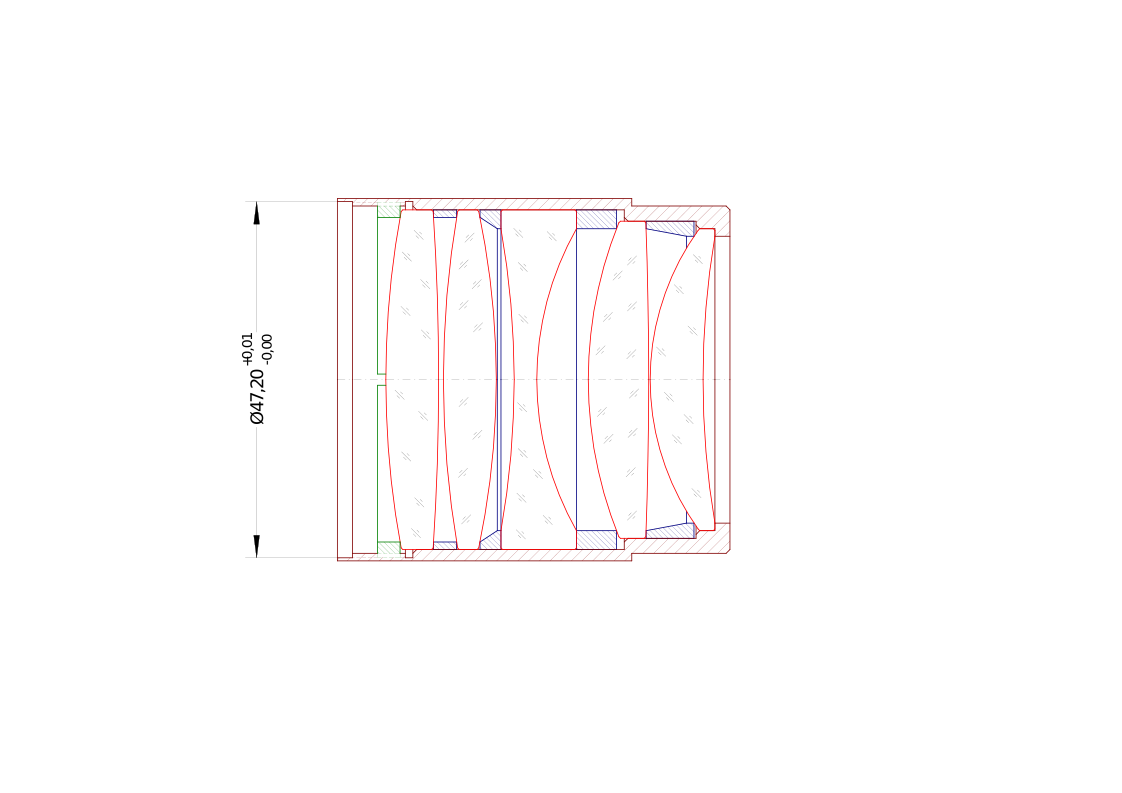
\includegraphics[width = \textwidth]{obj}
          \caption{Section of the custom objective, red parts are the lenses, while the rest is the housing.}
         \label{objsection}
     \end{subfigure}
     \hfill
     \begin{subfigure}[b]{0.55\textwidth}
         \centering
         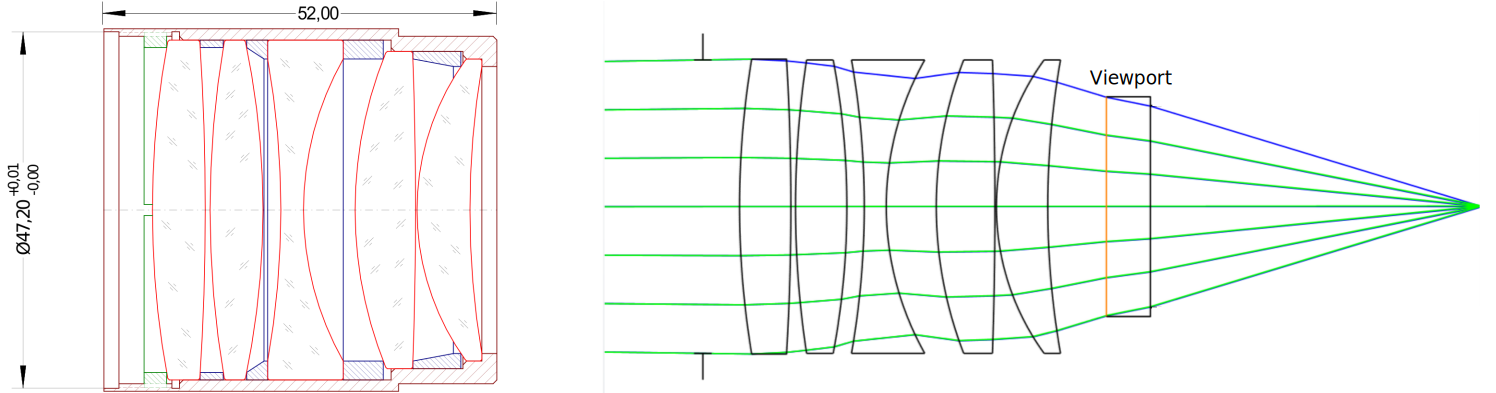
\includegraphics[width=\textwidth]{zeemaxobj}
         \vspace{1em}
         \caption{Zemax simulation of the objective. On the right, viewport and the vacuum chamber are also present.}
         %\label{fig:three sin x}

     \end{subfigure}
        \caption{}
      %  \label{fig:three graphs}
\end{figure}
The AOD is from Gooch \& Housego, model 4120-3. It has a specified central frequency of 120 MHz, with 50 MHz, bandwidth, so the driving frequency ranges from 95 to 145 MHz with a maximum RF power of 0.3 W. Therefore, the angle of deflection should be $\pm 0.86^{\circ}$ (:|).  In this bandwidth the diffraction efficiency should remain above 75 \% and have an average of 83 \%. Further light is lost as much as 3\% of due to insertion losses. The active aperture measures $3\times 3$ mm, and the polarization has to be horizontal when entering the AOD, while it gets rotated during diffraction, as the specified output polarization is vertical.

\section{Design simulation}
The setup in figure \ref{addressingsetup} has been simulated with the software Zemax. The simulation had the purpose of assessing the performance of the setup, i.e. checking the viability of the setup and see if it meets all requirements. It was also used to find the best lenses for building the setup and the best placement. Not everything was simulated, bu only the essential parts. This includes the four lenses, the objective, the viewport and the vacuum chamber. As there is no option to simulate an AOD, it was not taken in consideration, instead the simulation started at the output of the AOD as described below. Mirrors and beam splitters also do not alter drastically the optical path and therefore there was no need to simulate them.



\begin{figure}[H]
\centering
\includegraphics[width=\textwidth]{img/Plosses}
\caption{Losses on the compensation electrodes vs beam waist}
\end{figure}
\begin{figure}[H]
\centering
\includegraphics[width=\textwidth]{img/clipping}
\caption{Clipping on compensation electrodes}
\end{figure}

\section{Physical implementation}
- test setup
- picture
- alignment process



%More

\chapter{Experimental results}
\section{AOD}
\section{Full test setup characterisation}
\subsection{Test: razor blade and camera}
\begin{figure}[H]
\centering
\includegraphics[width=\textwidth]{img/prova7}
\caption{Example of razor scan}
\end{figure}
\begin{figure}[H]
\centering
\includegraphics[width=\textwidth]{img/camera}
\caption{Example of camera picture}
\end{figure}
\subsection{Polarization characterization}
\subsection{Stability}
\section{Final installed system}
\subsection{Ramsey interferometry}
\begin{figure}[H]
\centering
\includegraphics[width=\textwidth]{img/AODscan}
\caption{3 ions scanned}
\end{figure}
\begin{figure}[H]
\centering
\includegraphics[width=\textwidth]{img/ac_stark}
\caption{393nm AC-Stark flops}
\end{figure}

\subsection{Photons production}
\begin{figure}[H]
\centering
\includegraphics[width=\textwidth]{img/photonefficency_witherror}
\caption{Generated photon efficency}
\end{figure}

\begin{figure}[H]
\centering
\includegraphics[width=\textwidth]{img/ramanlength_witherrors}
\caption{Excitation of ion while emitting photon}
\end{figure}

- g2 plot?
\section{Final properties summary}

\chapter{Conclusions and outlook}
- Usual conclusions

\newpage
%\renewcommand\refname{References} % name for the reference list

\addcontentsline{toc}{section}{References} % to change the name of the references in the TOC
\bibliographystyle{plain}
\bibliography{References} % adds the references to the document


\newpage
\renewcommand{\appendixpagename}{Appendix} % Heading of appendix
\renewcommand{\appendixtocname}{Appendix} % name of appendix in TOC
\appendixpage
\addappheadtotoc


\begin{appendices}
- Error analysis? Maximum likehood estimation?
\end{appendices}

\end{document}
